\begin{figure}
    \centering
    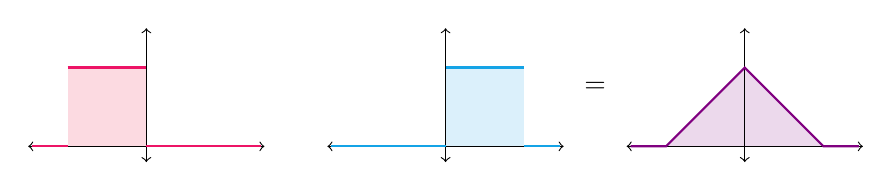
\begin{tikzpicture}
        \fill[WildStrawberry!15] (-1, 1) -- (0, 1) -- (0, 0) -- (-1, 0) -- cycle;

        \draw[<->] (-1.5, 0) -- (1.5, 0);
        \draw[<->] (0, -0.2) -- (0, 1.5);

        \draw[WildStrawberry, thick] (-1, 1) -- (0, 1);
        \draw[WildStrawberry, thick] (-1.45, 0) -- (-1, 0);
        \draw[WildStrawberry, thick] (0, 0) -- (1.45, 0);

        \node at (1.90, 0.75) {\( \convolution \)};

        \fill[Cerulean!15] (3.8, 1) -- (4.8, 1) -- (4.8, 0) -- (3.8, 0) -- cycle;

        \draw[<->] (2.3, 0) -- (5.3, 0);
        \draw[<->] (3.8, -0.2) -- (3.8, 1.5);

        \draw[Cerulean, thick] (3.8, 1) -- (4.8, 1);
        \draw[Cerulean, thick] (2.35, 0) -- (3.8, 0);
        \draw[Cerulean, thick] (4.8, 0) -- (5.25, 0);

        \node at (5.7, 0.75) {\( = \)};

        \fill[Purple!15] (6.6, 0) -- (7.6, 1) -- (8.6, 0) -- cycle;

        \draw[<->] (6.1, 0) -- (9.1, 0);
        \draw[<->] (7.6, -0.2) -- (7.6, 1.5);

        \draw[Purple, thick] (6.15, 0) -- (6.6, 0) -- (7.6, 1) -- (8.6, 0) -- (9.05, 0);
    \end{tikzpicture}
    \caption{When we take the convolution of the two uniform distributions, we get a "unit triangle" around \( x = 0 \).}
\end{figure}
